\documentclass[a4paper,11pt]{report}
\usepackage[T1]{fontenc}
\usepackage[utf8]{inputenc}
\usepackage[polish]{babel}
\usepackage{lmodern}
\usepackage{graphicx}

\title{Roznice w czasie realizacji algorytmow sortowania}
\author{Arkadiusz Cyktor 200367}

\begin{document}
\maketitle

\begin{figure}
  1. Ponizszy wykres przedstawia zaleznosc czasu potrzebnego na wykonanie algorytmu \textbf{quicksort}, jak widac rosnie ona wykladniczo.
   \begin{center} 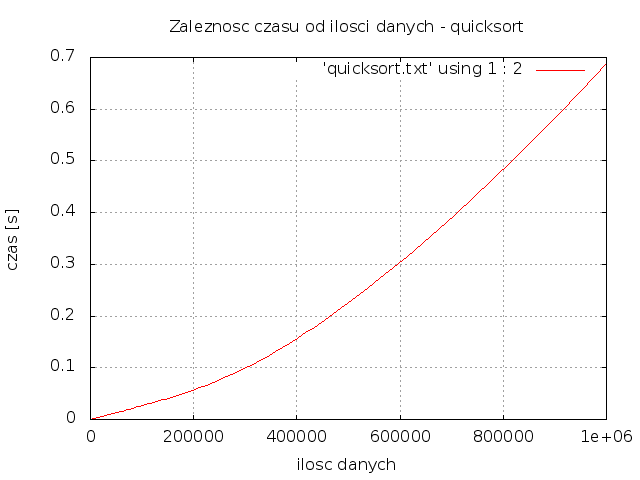
\includegraphics[scale=0.55]{./quicksort.png}\end{center}
   Teoretyczna srednia zlozonosc obliczeniowa tego algorytmu jest bliska zlozonosci w przypadku optymistycznym (wtedy gdy za kazdym razem udaje sie wybrac mediane z sortowanego fragmentu tablicy) i wynosi \emph{nlogn}. Wyniki moich testow, bardziej odpowiadaja przypadkowi pesymistycznemu, w ktorym wystepuje zlozonosc kwadratowa. Wynika to z faktu, ze przy liczbie powtorzen algorytmu wiekszej niz 1, sortowana bedzie posortowana juz tablica - przypadek pesymistyczny.
   Po zamianie liczby powtorzen na 1 zlozonosc zmienia sie wedlug zaleznosci \emph{nlogn}. W pewnym stopniu obrazuje to ponizszy wykres.
   \end{figure}


\begin{figure}
\begin{center} 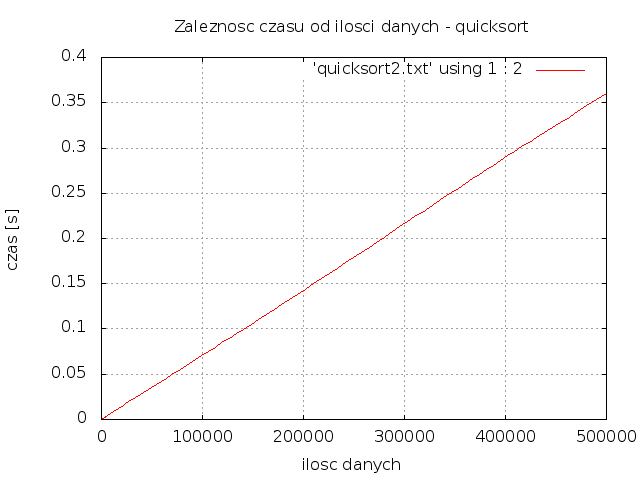
\includegraphics[scale=0.55]{./quicksort2.png}\end{center}
  2. Ponizszy wykres przedstawia zaleznosc czasu potrzebnego na wykonanie algorytmu \textbf{heapsort}.
    \begin{center}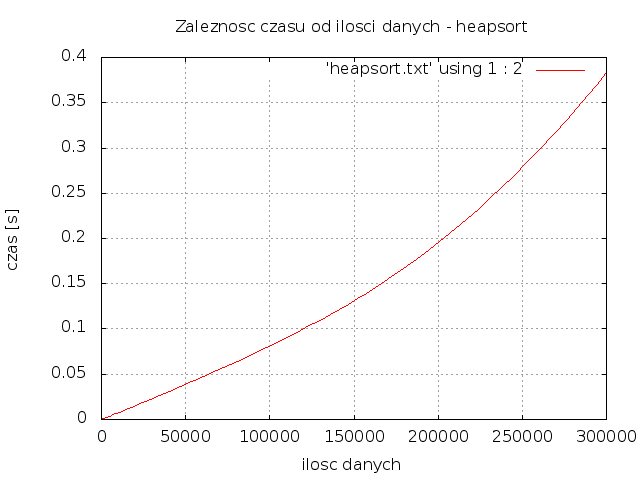
\includegraphics[scale=0.55]{./heapsort.png}\end{center}
    \end{figure}

\begin{figure}
    Jak, moze niezbyt dobrze, widac na wykresie - zlozonosc obliczeniowa zmienia sie wedlug zaleznosci \emph{nlogn}, co odpowiada pesymistycznemu przypadkowi dla tego algorytmu (kazde wstawienie nowego elementu na stos wymaga tylu przesuniec, ile jest wezlow na sciezce od miejsca wstawienia do korzenia drzewa). Po zmianie liczby powtorzen na 1 otrzymalem zaleznosc liniowa - \emph{n}, wiec testowany przypadek byl optymistyczny (dodanie nowego elementu nie naruszalo struktury kopca).
     \begin{center}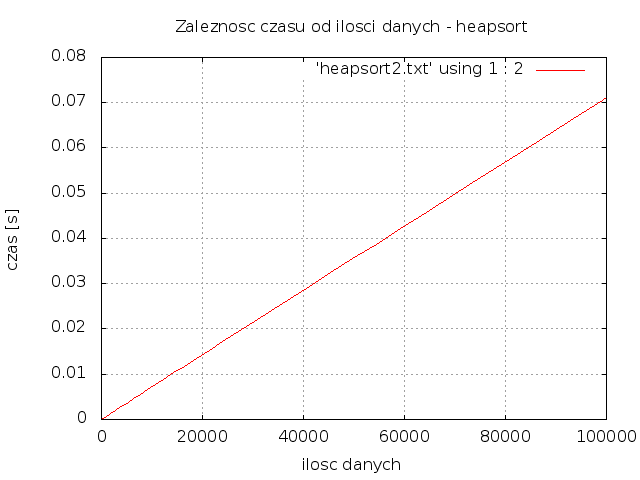
\includegraphics[scale=0.55]{./heapsort2.png}\end{center}
\end{figure}

\begin{figure}
  3. Ponizszy wykres przedstawia zaleznosc czasu potrzebnego na wykonanie algorytmu \textbf{mergesort}. Algorytm ten charakteryzuje sie taka sama zlozonoscia obliczeniowa dla kazdego przypadku - wynosi ona \emph{nlogn}. Obrazuje to ponizszy wykres (zaleznosc \emph{nlogn} latwo pomylic z wykladnicza, zwlaszcza w przypadku takim jak ten - gdy z oczywistych wzgledow os \emph{y} nie przyjmuje wartosci ujemnych).
   \begin{center} 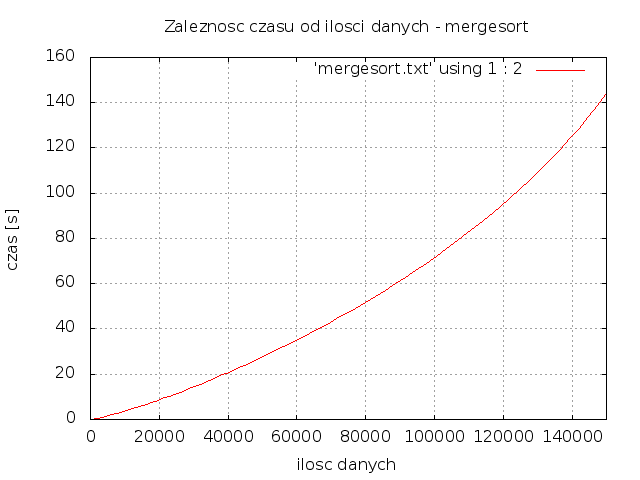
\includegraphics[scale=0.55]{./mergesort.png}\end{center}
\end{figure}
\end{document}
